\section{Data} \label{tex:data}

In this thesis two different data sets will be used; the well-studied MNIST data set \cite{MNIST} of handwritten digits, and the relatively new THETIS data set \cite{Gourgari2013} of videos of tennis shots. The idea is to first apply the methods discussed later to the simpler MNIST data set, to make sure that it is working properly, followed by an application to the more complicated THETIS data set. This also makes it possible to examine the potentially different effect the methods discussed later will have on the speed-up. Each of the data sets will be described in the following. 

\subsection{MNIST - Handwritten Digits}
The MNIST (Modified National Institute of Standards and Technology) data set \cite{MNIST} consists of 70,000 pictures\footnote{The 70,000 is split into 60,000 training pictures and 10,000 testing pictures} of handwritten digits from 0 through 9. Each picture is $28\times 28$ pixels and black/white which means that there is only one input channel. Each of the $28\cdot 28 = 784$ pixel values are intensities ranging from 0 (black) to 255 (white). The data set is formed by remixing samples from the earlier NIST data set, which consisted of both digits and characters. The MNIST samples would be picked out, standardized and normalized so they would all be the same size and have the same gray-values \cite{mnistdatabase}. The first 175 samples from the traning set of the MNIST database is shown in \autoref{fig:MNISTdata175}. 

\begin{figure}[H]
    \centering
    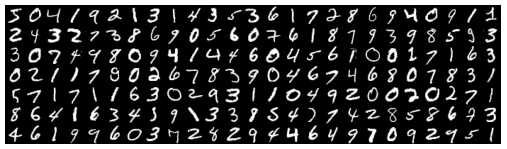
\includegraphics[width=\linewidth]{Pics/04_Data/MNIST.png}
    \caption{The first 175 samples of the MNIST data set of handwritten digits}
    \label{fig:MNISTdata175}
\end{figure}

\subsection{THETIS - Tennis Shot Videos}
The THETIS (Three dimEnsional TennIs Shots) data set consists of videos of 1980 tennis shots performed by both beginners and more experienced individuals \cite{Gourgari2013}. Each of the 12 shots types have been performed multiple times by each of the 55 individuals (31 beginners and 24 experts). Each shot consists of an RGB video, a depth video, a silhouette video, and both 2D and 3D skeleton videos. The videos have a resolution of $480\times 640$, while they vary in length (approximately 3-7 s). Since the skeleton extraction is not always successful, only 1217 of the shots have this feature. This means that the total number of videos in the data set is 8,374 resulting in a total playtime of 7 hours and 15 minutes. An overview of the 12 types of shots is given in \autoref{tab:typeOverviewTHETIS}, while an example of each of the five features is given in \autoref{fig:exampleVideosTennis}. 

\begin{table}
\centering
\caption{Overview of the 12 different types of tennis shots present in the THETIS data set.}
\label{tab:typeOverviewTHETIS}
\begin{tabular}{l|l|l|l}
\textbf{Forehand}    & \textbf{Backhand}     & \textbf{Service} & \textbf{Other} \\ \hline
Flat        & With 2 hands & Flat    & Smash \\
Slice       & Slice        & Slice   &       \\
Volley      & Volley       & Kick    &       \\
Open stands & Backhand     &         &      
\end{tabular}
\end{table}

\begin{figure}
    \centering
    \begin{subfigure}{.49\linewidth}
        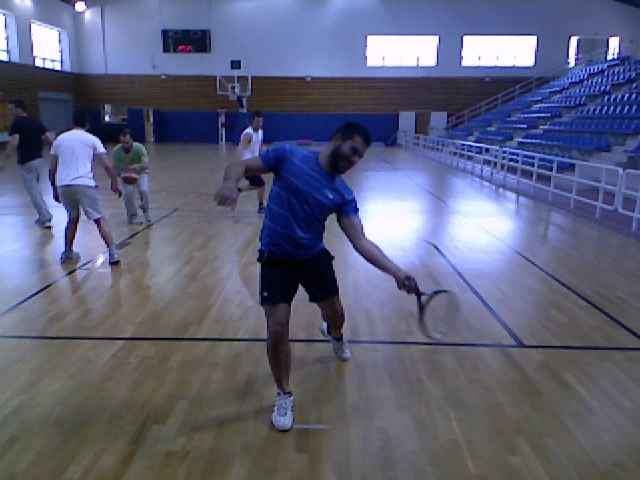
\includegraphics[width=\linewidth]{Pics/04_Data/frame53.jpg}
        \caption{Normal RGB video}
    \end{subfigure}
    \begin{subfigure}{.49\linewidth}
        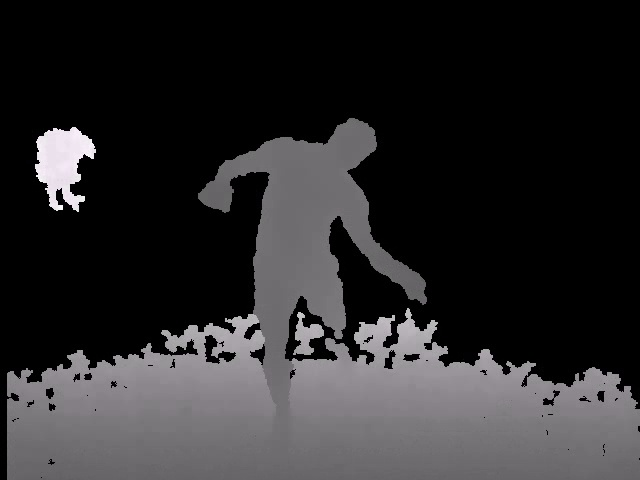
\includegraphics[width=\linewidth]{Pics/04_Data/frame53_depth.jpg}
        \caption{Depth video}
    \end{subfigure}
    \begin{subfigure}{.32\linewidth}
        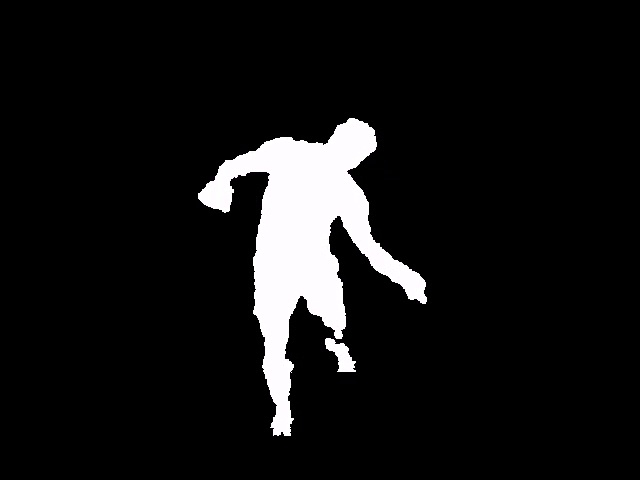
\includegraphics[width=\linewidth]{Pics/04_Data/frame53_mask.jpg}
        \caption{Silhouette}
    \end{subfigure}
    \begin{subfigure}{.32\linewidth}
        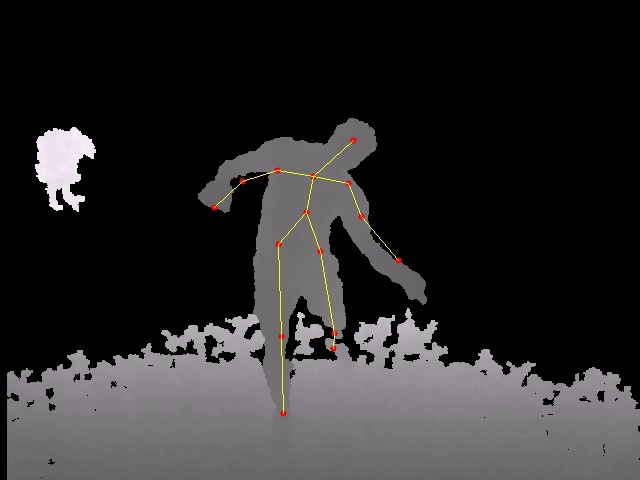
\includegraphics[width=\linewidth]{Pics/04_Data/frame53_skelet2D.jpg}
        \caption{2D Skeleton}
    \end{subfigure}
    \begin{subfigure}{.32\linewidth}
        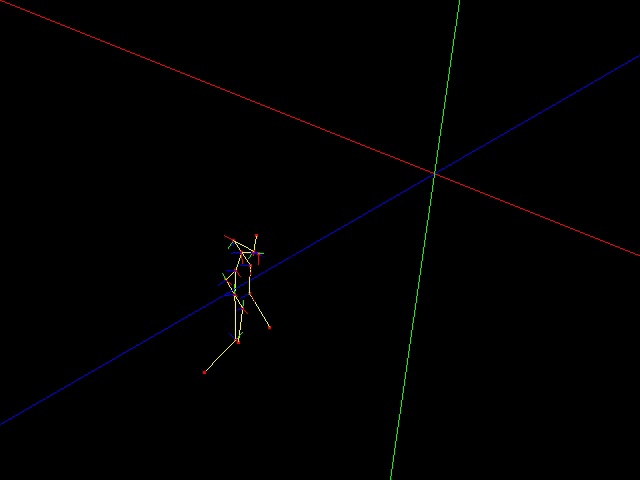
\includegraphics[width=\linewidth]{Pics/04_Data/frame53_skelet3D.jpg}
        \caption{3D skeleton}
    \end{subfigure}
    \caption{Example of the different videos that are given for each shot in the data set. Each of the pictures show the same frame in each of the videos of the same shot. Note that the 3D skeleton looks different since this is shown from a different angle. The 3D skeleton joint positions are also given numerically for each frame in the whole dataset.}
    \label{fig:exampleVideosTennis}
\end{figure}

Even though this data set is quite simple in relation to the real world, it is still complicated, especially relative to the MNIST data set. The videos feature different individuals - both men and women, right handed and left handed, professionals and beginners. Even though the same type of shot is being performed by two individuals, they can look very different from each other. Also some of the videos are recorded in a sports arena with people doing different activities in the background as for instance yoga or basketball, while the others are recorded in a changing room with no visual noise.

\subsubsection{Pre-processing for THETIS}
In order to properly train on the THETIS data set, some preprocessing is needed. It is desirable to have the videos scaled down both in space and time, and to use more than just the RGB video from the data set. The depth video, which shows the depth information of the video on a gray-scale, only has one channel, and was easy to concatenate onto the RGB videos. This make the data set now have 4 input channels, which means more information to train on. The 4 channels of a single frame in the data set is illustrated in \autoref{fig:video_data_frame}. 
\begin{figure}
    \centering
    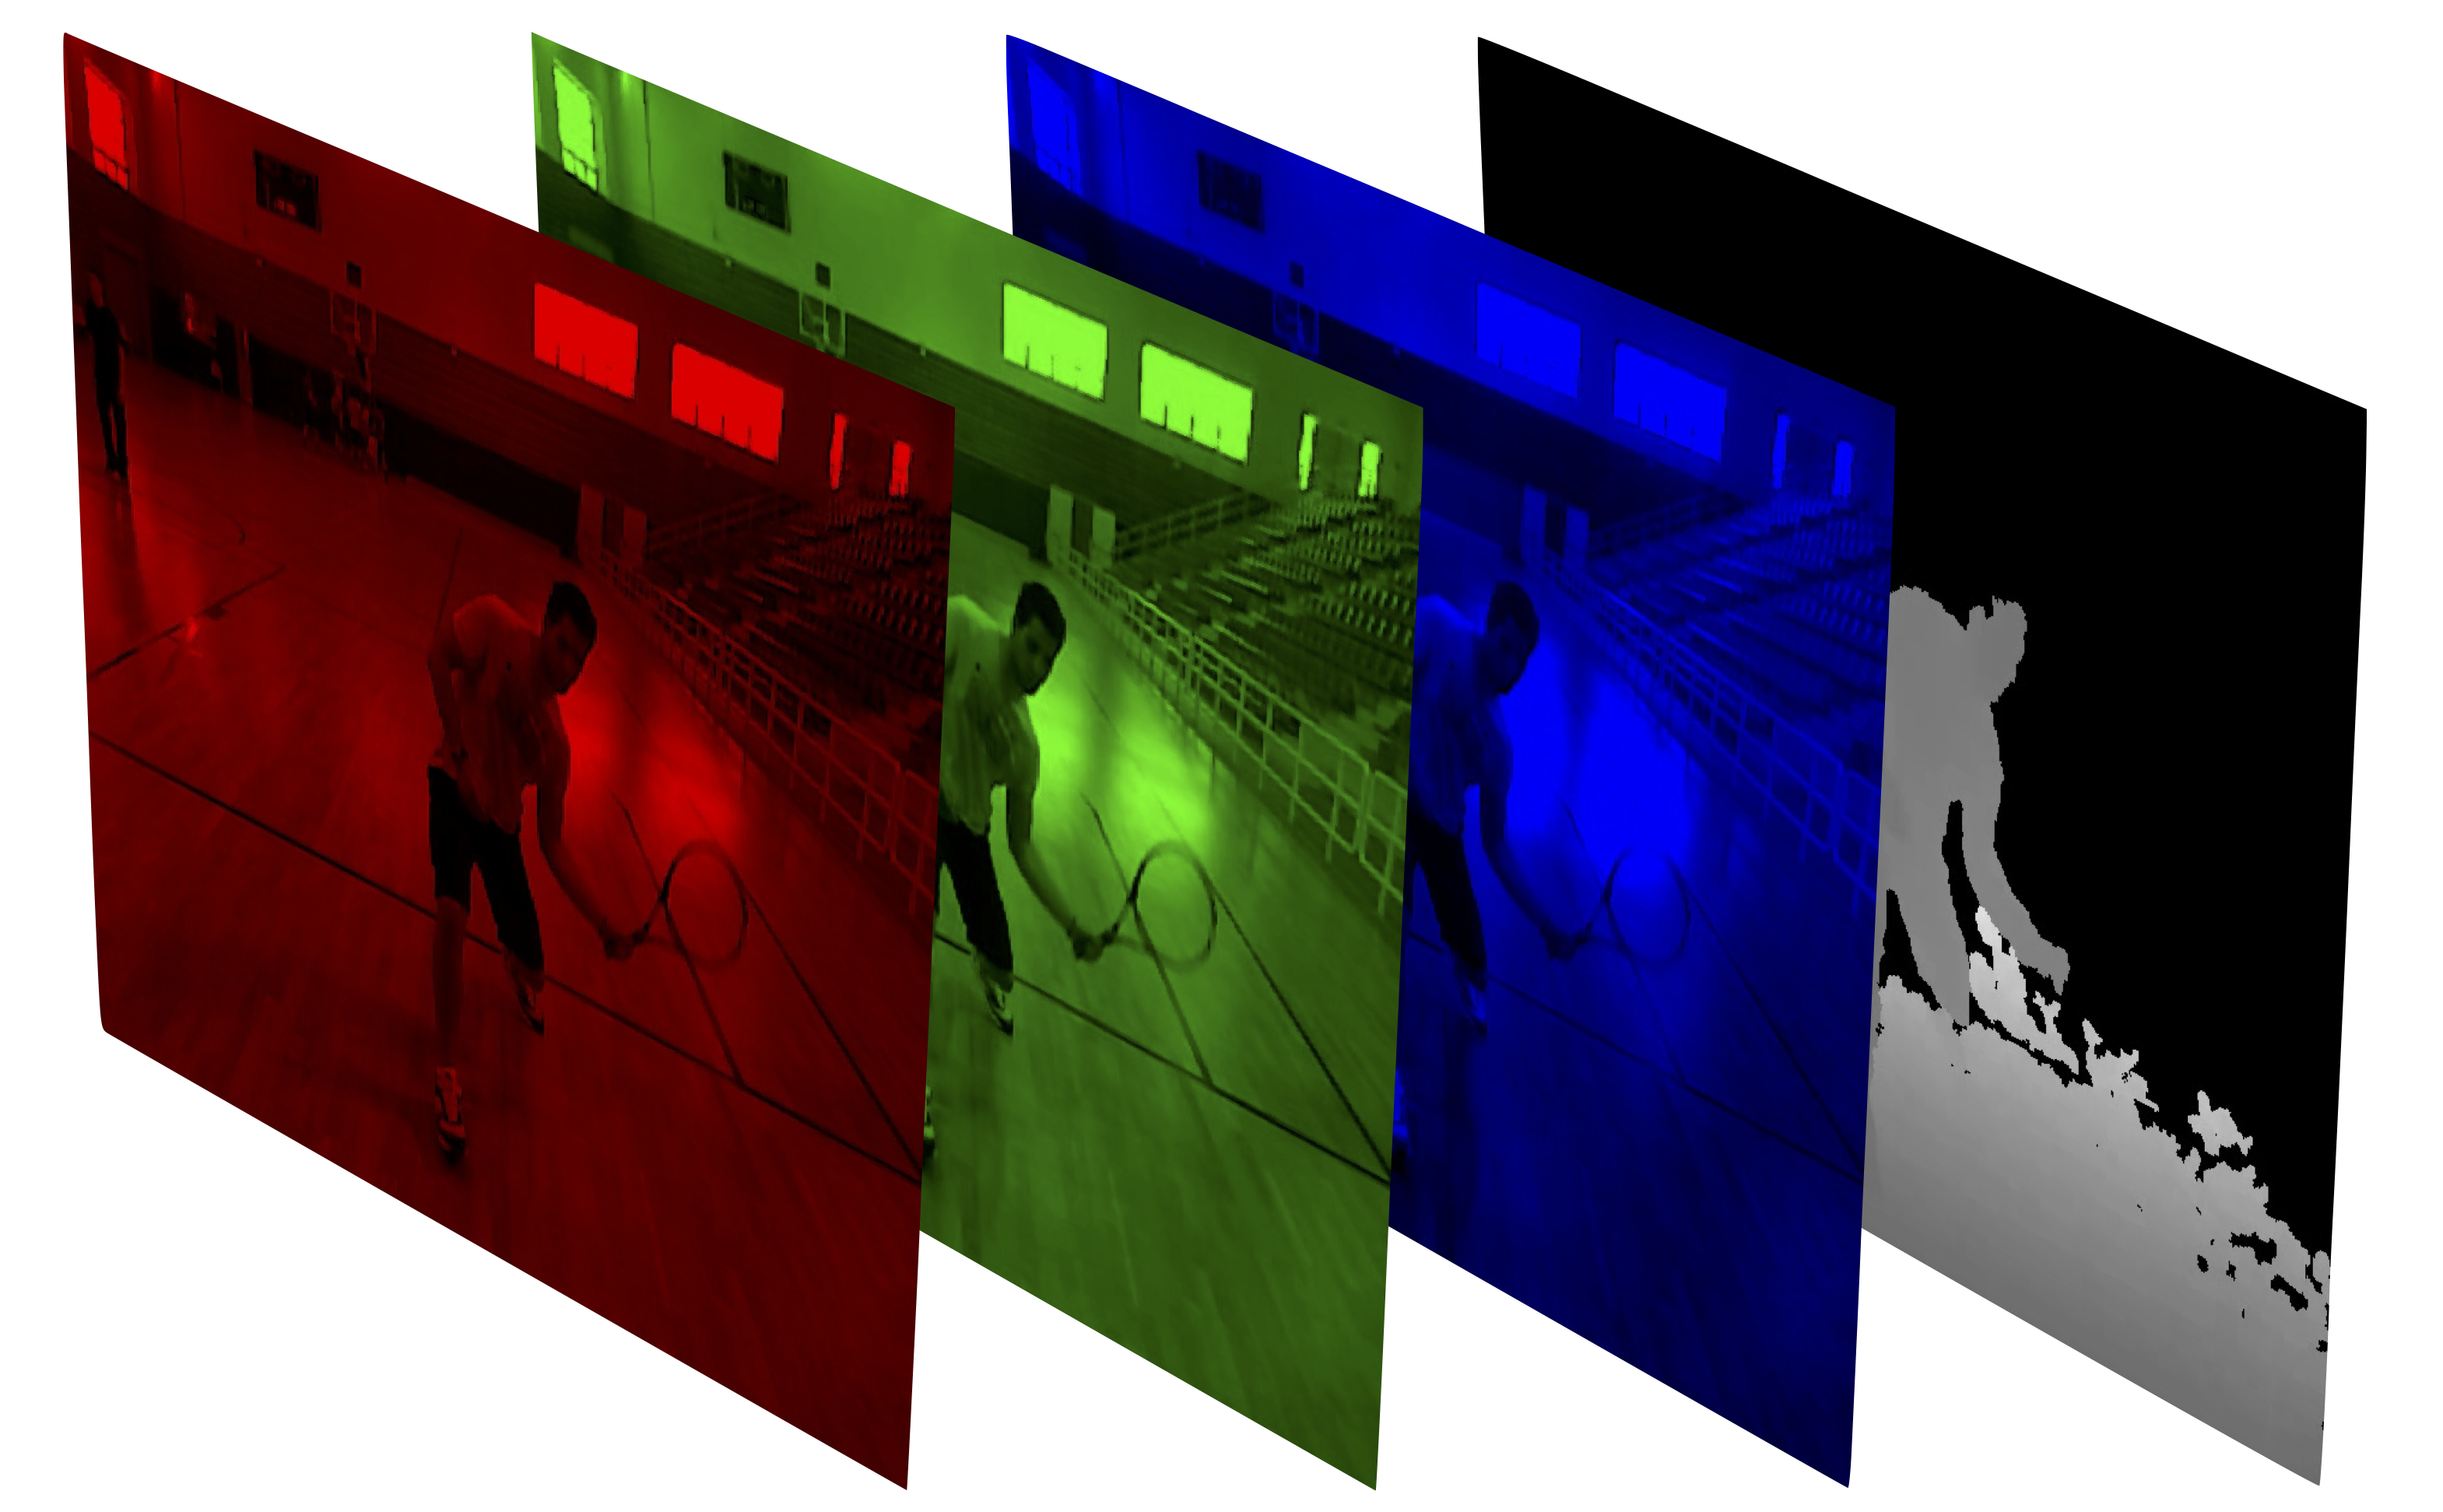
\includegraphics[width=.9\linewidth]{Pics/04_Data/RGBD.png}
    \caption{Each frame of the videos consists of 4 input channels; one red, one green, one blue, and one depth channel.}
    \label{fig:video_data_frame}
\end{figure}

One of the problems is that all the videos input into the network needs to have the same size, hence also the same length (number of frames). How this is typically ensured is by splitting the video into smaller pieces of the same length, and then running the algorithm on all the pieces and letting the majority of the smaller videos determine the class.\cite{Karpathy2014} While this is appropriate when trying to classify a general activity like running, swimming etc., it does not seem appropriate for this problem. This is due to the tennis shots being performed once per video, making the whole sequence a part of the shot. The problem was solved by manually inspecting the videos and assigning the time for the approximate midway through the shot. The assigned times are then used to extract the same number of frames on either side of the midway, making all videos have the same number of frames. This also has a standardizing effect, due to the middle of the shot being at the approximate same time in all videos. The number of frames is experimentally set to 14, making all videos 28 frames.

The last thing that was done to the data, was to decrease the resolution by a factor of 4 in each spatial dimension, i.e. from a resolution of $480\times 640$ to a resolution of $120\times 160$. This results in the number of pixels decreasing by a factor of 16 from 307,200 to 19,200, while still having a relatively high resolution that should be fine to train on. 

Due to the complexity of the problem only the videos depicting a back-hand or a forehand flat shot is considered. This means that there will be a total of 327 videos with approximately equal distributions of the two types of shot. The low amount of data means that cross-validation will be used to carry out the training.

All of the above results in the 327 THETIS observations having the size \begin{equation}
    (S \times F \times H \times W) = 4\times 28 \times 120 \times 160
\end{equation}
Where $S$ is the input channels, $F$ is the number of frames, $H$ is the height in pixels, and $W$ is the width in pixels.